%%%%%%%%%%%%%%%%%%%%%%%%%%%%%%%%%%%%%%%%%
% Focus Beamer Presentation
% LaTeX Template
% Version 1.0 (8/8/18)
%
% This template has been downloaded from:
% http://www.LaTeXTemplates.com
%
% Original author:
% Pasquale Africa (https://github.com/elauksap/focus-beamertheme) with modifications by 
% Vel (vel@LaTeXTemplates.com)
%
% Template license:
% GNU GPL v3.0 License
%
% Important note:
% The bibliography/references need to be compiled with BibTeX.
%
%%%%%%%%%%%%%%%%%%%%%%%%%%%%%%%%%%%%%%%%%
% https://www.latextemplates.com/template/focus-presentation

%----------------------------------------------------------------------------------------
% PACKAGES AND OTHER DOCUMENT CONFIGURATIONS
%----------------------------------------------------------------------------------------

\documentclass[9pt]{beamer}
\usepackage[ngerman]{babel}
\usepackage{catchfile}                      % used for gitHash extraction
\usepackage{xstring}                        % used for gitHash extraction

\usetheme{focus}

% Git hash extraction and custom cmd
\CatchFileDef{\headfull}{../.git/HEAD.}{}
\StrGobbleRight{\headfull}{1}[\head]
\StrBehind[2]{\head}{/}[\branch]
\IfFileExists{../.git/refs/heads/\branch.}{%
    \CatchFileDef{\commit}{../.git/refs/heads/\branch.}{}}{%
    \newcommand{\commit}{\dots~(in \emph{packed-refs})}}

\usepackage{booktabs} % Required for better table rules

% Change display spacing
\newcommand{\zerodisplayskips}{%
    \setlength{\abovedisplayskip}{-5pt}
    \setlength{\belowdisplayskip}{0pt}}
\appto{\normalsize}{\zerodisplayskips}

\title{Optische Fouriertransformation}
\subtitle{MathSem 2023}
\author{Marco Niederberger \texorpdfstring{\\}{} Yanick Schoch}
\titlegraphic{\includegraphics[scale=0.5]{../../SeminarHarmonischeAnalysis/buch/papers/opt/images/jamesWebb_cropped_publicDomain.png}} % Optional title page image, comment this line to remove it
\institute{OST - Ostschweizer Fachhochschule}
\date{08. Mai 2023}

\begin{document}

% Steady screen for start
\begin{frame}[plain]
    \begin{tikzpicture}[overlay, remember picture]
        \node[inner sep=0pt] at (current page.center)
        {\includegraphics[height=\pdfpageheight]{../../SeminarHarmonischeAnalysis/buch/papers/opt/images/jamesWebb_publicDomain.png}};
    \end{tikzpicture}
\end{frame}

\begin{frame}[noframenumbering]
    \maketitle % Automatically created using the information in the commands above
\end{frame}

% Overview
\begin{frame}<1>[label=opt:goals]{Heutige Ziele}
    \begin{block}<1->{\strut \only<3>{Ziele erreicht?}}
        \begin{itemize}
            \item Was ist Beugung?
            \item Woher kommt die Fouriertransformation?
            \item Wie geht das praktisch?
            \item Für was ist das nützlich?
        \end{itemize}
    \end{block}
\end{frame}

% Sections
\section{Grundlagen}

\begin{frame}{Grundlagen - Beugung von Wellen}
    \centering
    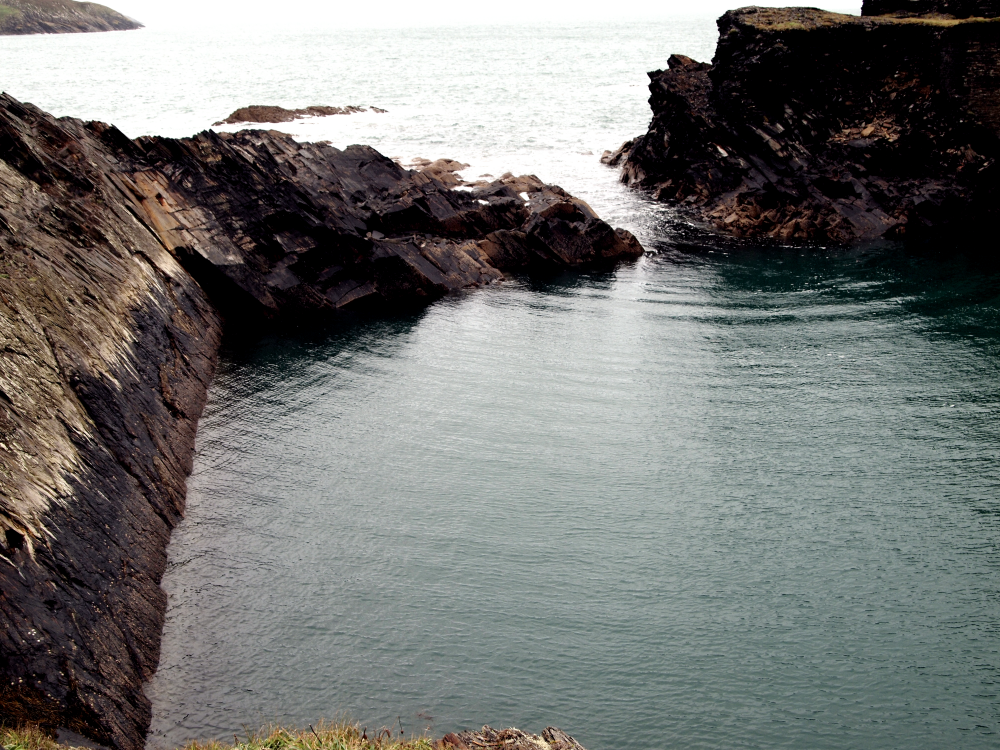
\includegraphics[width=0.9\linewidth]{images/beugung_von_wasserwellen.png}
\end{frame}

\begin{frame}{Grundlagen - Prinzip von Huygens}
    \includegraphics[width=\linewidth]{../../SeminarHarmonischeAnalysis/buch/papers/opt/images/huygens.pdf}
\end{frame}

\begin{frame}{Grundlagen - Beugung beim JWST}
    \begin{columns}
        \begin{column}{0.5\textwidth}
            \centering
            \includegraphics[width=\textwidth, page = 1]{../../SeminarHarmonischeAnalysis/buch/papers/opt/images/jwst_sechseck.pdf}
            Beugung am Spiegel
        \end{column}
        \pause
        \begin{column}{0.5\textwidth}
            \centering
            \includegraphics[width=\textwidth, page = 2]{../../SeminarHarmonischeAnalysis/buch/papers/opt/images/jwst_sechseck.pdf}
            Beugung an den Streben
        \end{column}
    \end{columns}
\end{frame}

\begin{frame}[plain]
    \begin{tikzpicture}[overlay, remember picture]
        \node[inner sep=0pt] at (current page.center)
        {\includegraphics[height=\pdfpageheight]{../../SeminarHarmonischeAnalysis/buch/papers/opt/images/jamesWebb_publicDomain.png}};
    \end{tikzpicture}
\end{frame}

\begin{frame}{Grundlagen - Wellendarstellung}
    \begin{center}
        \includegraphics[width=0.7\linewidth]{../../SeminarHarmonischeAnalysis/buch/papers/opt/images/welle.pdf}
    \end{center}
    \begin{equation*}
        \zeta(x, t)
        =
        \zeta_0 \cdot e^{j(\omega t - \vec{k}\cdot\vec{x})}
    \end{equation*}
    \begin{equation*}
        k
        =
        \frac{\omega}{u}
        =
        \frac{2 \pi}{\lambda}
    \end{equation*}
\end{frame}

\begin{frame}{Grundlagen - Maxwell}
    \begin{columns}
        \begin{column}{0.5\textwidth}
            \begin{center}
                \includegraphics[width=\linewidth]{../../SeminarHarmonischeAnalysis/buch/papers/opt/images/maxwell.pdf}
            \end{center}
        \end{column}

        \begin{column}{0.5\textwidth}
            \pause
            \begin{block}{Block}
                \begin{align*}
                    \oint_{S=\partial V} \varepsilon\vec{E} \cdot\, d\vec{S}
                    &=
                    \int_{V}\rho\, dV
                    \\
                    \int_{0}^{a}\int_{0}^{2\pi} \varepsilon E\cdot 1 \cdot r\, d\varphi dl
                    &=
                    Q
                    \\
                    2\pi ra\varepsilon E
                    &=
                    Q
                \end{align*}
            \end{block}
            \pause
            \begin{exampleblock}{dfasdf Example block}
                \begin{equation*}
                    E(r)
                    =
                    \frac{Q}{2\pi\varepsilon a} \cdot \frac{1}{r}
                    =
                    C \cdot \frac{1}{r}
                \end{equation*}
            \end{exampleblock}
        \end{column}
    \end{columns}
\end{frame}

\begin{frame}{Grundlagen - Beugungsintegral}
    \begin{center}
        \includegraphics[width=0.7\linewidth]{../../SeminarHarmonischeAnalysis/buch/papers/opt/images/derivation.pdf}
    \end{center}
    % \begin{equation*}
    %     E(y_p, t)
    %     =
    %     C\zeta_0 \cdot \int_{-\infty}^{\infty}f(y)\cdot\frac{e^{j(\omega t - \vec{k}\cdot\vec{r})}}{r} \,dy
    % \end{equation*}
    \begin{equation}
        dE
        =
        E(r) \cdot \zeta(r, t) \cdot dy
        =
        \frac{C}{r} \cdot \zeta_0 \cdot e^{j(\omega t - \vec{k}\cdot\vec{r})} \cdot dy
    \end{equation}
\end{frame}

\begin{frame}{Approximation - Fresnel}
    \begin{columns}
        \begin{column}{0.4\textwidth}
            \centering
            \includegraphics[width=\linewidth]{../../SeminarHarmonischeAnalysis/buch/papers/opt/images/derivation.pdf}
        \end{column}

        \begin{column}<1->{0.6\textwidth}
            \begin{block}<1->{Binominalexpansion}
                \begin{equation*}
                    (1+\varepsilon)^n \approx 1 + n\varepsilon \text{ für } \varepsilon \ll 1
                \end{equation*}
            \end{block}
            \begin{block}<2->{Angewandt}
                \begin{equation*}
                    r
                    =
                    l \sqrt{1 + \alert{\frac{(y_p-y)^2}{l^2}}}
                    =
                    l \biggl(1 + \alert{\frac{(y_p-y)^2}{l^2}}\biggr)^{-\frac{1}{2}}
                \end{equation*}
                \begin{equation*}
                    r
                    \approx
                    l \left(1 \alert{-} \frac{(y_p-y)^2}{\alert{2}l^2}\right)
                    =
                    l - \frac{(y_p-y)^2}{2l}
                \end{equation*}
            \end{block}
            \begin{block}<3->{Einsetzen ins Beugungsintegral}
                \begin{equation*}
                    E(y_p, t)
                    =
                    C\zeta_0 \cdot e^{j\omega t} \cdot \int_{-\infty}^{\infty}f(y)\cdot\frac{e^{-j\vec{k}\cdot\vec{r}}}{r} \,dy
                \end{equation*}
            \end{block}
        \end{column}
    \end{columns}
\end{frame}

\begin{frame}{Approximation - Fresnel}
    \begin{block}<1->{Einsetzen ins Beugungsintegral (cont.)}
        \begin{align*}
            E(y_p, t)
            &=
            C\zeta_0 \cdot e^{j\omega t} \cdot \int_{-\infty}^{\infty}f(y)\cdot\frac{e^{-j\vec{k}\cdot\vec{r}}}{r} \,dy \\
            &=
            C\zeta_0 \cdot e^{j\omega t} \cdot \int_{-\infty}^{\infty}f(y)\cdot\frac{e^{-jkl} \cdot e^{jk\frac{(y_p-y)^2}{2l}}}{l - \frac{(y_p-y)^2}{2l}} \,dy \\
            E(y_p, t = 0)
            &=
            C\zeta_0 \cdot e^{j\omega t} \cdot e^{-jkl} \cdot \int_{-\infty}^{\infty}f(y)\cdot\frac{e^{jk\frac{(y_p-y)^2}{2l}}}{l} \,dy \\
        \end{align*}
    \end{block}
    \begin{exampleblock}<2->{Fresnelapproximation}
        \begin{equation*}
            E(y_p, t)
            =
            \frac{C\zeta_0}{l} \cdot e^{-jkl} \cdot \int_{-\infty}^{\infty}f(y)\cdot e^{jk\frac{(y_p^2 - 2y_py + y^2)}{2l}} \,dy
        \end{equation*}
    \end{exampleblock}
\end{frame}

\begin{frame}{Approximation - Fraunhofer}
    \begin{block}<1->{Weiter vereinfachen im Fernfeld}
        \begin{equation*}
            E(y_p, t)
            =
            \frac{C\zeta_0}{l} \cdot e^{-jkl} \cdot \int_{-\infty}^{\infty}f(y)\cdot e^{jk\frac{(\alert{y_p^2 - 2y_py + y^2})}{2l}} \,dy
        \end{equation*}
        \begin{equation*}
            \text{mit }
            y
            \ll
            y_p
            \ll
            l
            \text{ kann }
            y^2
            \text{ vernachlässigt werden}
        \end{equation*}
    \end{block}
    \begin{block}<2->{Einsetzen in die Fresnelapproximation}
        \begin{align*}
            E(y_p)
            &=
            \frac{C\zeta_0}{l} \cdot e^{-jkl} \cdot \int_{-\infty}^{\infty}f(y)\cdot e^{jk\frac{(y_p^2 - 2y_py)}{2l}} \,dy
            \\
            &=
            \frac{C\zeta_0}{l} \cdot e^{-jk\left(l-\frac{y_p^2}{2l}\right)} \cdot \int_{-\infty}^{\infty}f(y)\cdot e^{-j\frac{ky_p}{l}y} \,dy
        \end{align*}
    \end{block}
    \begin{exampleblock}<3->{Fouriertransformation}
        \begin{align*}
            E(y_p)
            &=
            C \cdot \int_{-\infty}^{\infty}f(y)\cdot e^{-jy_py} \,dy
        \end{align*}
    \end{exampleblock}
\end{frame}

\section{Versuch}

\begin{frame}{Versuch - Laser aufweiten}
    \centering
    \includegraphics[width = 0.5\textwidth]{../../SeminarHarmonischeAnalysis/buch/papers/opt/images/laserAufweiten.pdf}
\end{frame}

\begin{frame}{Versuch - 4f Aufbau}
    \includegraphics[width = \textwidth]{../../SeminarHarmonischeAnalysis/buch/papers/opt/images/4fAufbau.pdf}
\end{frame}

\section{Anwendungen}

% \begin{frame}<1-3>[label=opt:patternMatching]{Anwendungen - Pattern matching}
%     \begin{block}<1->{Muster im Spektrum detektieren}
%         \begin{itemize}
%             \item<1-> Jeden Input gibt eine Fouriertransformation
%             \item<1-> Unterschiedliche Muster - unterschiedliches Spektrum
%             \item<2-> Maskieren des gewünschten Spektrums
%             \item<3-> Helligkeitsmessung nach der Maske
%         \end{itemize}
%     \end{block}
%     \begin{block}<4->{Optik statt Elektronik}
%         \begin{itemize}
%             \item<4-> Linsen statt Prozessor
%             \item<5-> $60 cm$ Distanz plus $100 ps$ Anstiegszeit der Photodiode
%             \begin{itemize}
%                 \item $\frac{0.6 m \cdot s^{-1}}{3 \cdot 10^8 m} = 2 ns$
%                 \item $\frac{1}{2.1 ns = 1 ns} \approx 0.5 GHz$
%             \end{itemize}
%         \end{itemize}
%     \end{block}
% \end{frame}

% \begin{frame}{Anwendungen - Pattern matching}
%     \centering
%     \includegraphics[width = 0.8\textwidth]{../../SeminarHarmonischeAnalysis/buch/papers/opt/images/pattern_YT.png}
%     \vfill
%     Youtube: Huygens Optics \cite{opt:YT:PatternRecognition}
% \end{frame}

% \againframe<4->{opt:patternMatching}

\begin{frame}{Anwendungen - Diffractive deep neural network}
    \centering
    \includegraphics[width = 0.8\textwidth]{../../SeminarHarmonischeAnalysis/buch/papers/opt/images/handwriting_xing.png}
    \vfill
    Xing et al. \cite{opt:Lin.2018}
\end{frame}

\begin{frame}{Anwendungen - Diffractive deep neural network}
    \centering
    \begin{columns}
        \column{0.4\textwidth}
        \includegraphics[width = 1\textwidth]{../../SeminarHarmonischeAnalysis/buch/papers/opt/images/handwriting_5_input_xing.png}
        Input
        \column{0.4\textwidth}
        \includegraphics[width = 1\textwidth]{../../SeminarHarmonischeAnalysis/buch/papers/opt/images/handwriting_5_output_xing.png}
        Output
    \end{columns}
\end{frame}

% \begin{frame}<1->[label=opt:deepLearning]{Anwendungen - Diffractive deep neural network}
%     \begin{block}<1->{Aktuelle Forschung}
%         \begin{itemize}
%             \item<1-> Handschrifterkennung mit Beugung
%             \item<1-> Fünf Beugungsebenen
%             \item<1-> Zehn Detektoren
%             \item<1-> 90\% Erfolgsrate
%         \end{itemize}
%     \end{block}
%     \begin{block}<2->{Vorteile}
%         \begin{itemize}
%             \item<2-> Geschwindigkeit
%             \item<2-> Parallelisierbar
%         \end{itemize}
%     \end{block}
% \end{frame}


\againframe<2-3>{opt:goals}

\begin{frame}[noframenumbering]
    \begin{tikzpicture}[overlay, remember picture]
        \node[inner sep=0pt] at (current page.center)
        {\includegraphics[height=\pdfpageheight]{../../SeminarHarmonischeAnalysis/buch/papers/opt/images/jamesWebb_publicDomain.png}};
    \end{tikzpicture}
\end{frame}

\appendix

\begin{frame}{Appendix - Referenzen}
    \nocite{*} % Display all references regardless of if they were cited
    \bibliography{example.bib}
    \bibliographystyle{plain}
\end{frame}

\begin{frame}{Appendix - Bildquellen}
    Beugung von Wasserwellen: \\
    \url{https://www.rhetos.de/html/lex/beugung_von_wasserwellen.htm}
\end{frame}

\begin{frame}{Appendix - Hintergrundinformationen}
    \begin{itemize}
        \item \LaTeX{} Präsentation mit dem Theme \emph{Focus}
    \end{itemize}

\end{frame}

\begin{frame}{Appendix - Wellenlängen}
    \begin{table}
        \centering % Centre the table on the slide
        \begin{tabular}{l c}
            \toprule
            Lichtfarbe & Wellenlänge in nm \\
            \toprule
            Violett    & $380 - 420$       \\
            Blau       & $420 - 490$       \\
            Grün       & $490 - 575$       \\
            Gelb       & $575 - 585$       \\
            Orange     & $585 - 650$       \\
            Rot        & $650 - 780$       \\
            \bottomrule
        \end{tabular}
        \caption{Wellenlänge von sichtbarem Licht}
    \end{table}
\end{frame}


\end{document}
